% Academic Research Report for Scaffold AI
% No external images are included; the TikZ figure is generated inline via input.
\documentclass[11pt]{article}
\usepackage[margin=1in]{geometry}
\usepackage{lmodern}
\usepackage[T1]{fontenc}
\usepackage{microtype}
\usepackage{setspace}
\usepackage{hyperref}
\usepackage{graphicx}
\usepackage{xcolor}
\usepackage{booktabs}
\usepackage{longtable}
\usepackage{enumitem}
\usepackage{tikz}
\usetikzlibrary{arrows.meta, positioning}

\hypersetup{
  colorlinks=true,
  linkcolor=black,
  citecolor=black,
  urlcolor=blue
}

\title{Integrating Sustainability and Climate Resilience into STEM with Scaffold AI: System Status Report}
\author{Scaffold AI Team}
\date{September 2025}

\begin{document}
\maketitle

\begin{abstract}
This report presents the current status of \emph{Scaffold AI}, a retrieval-augmented generation (RAG) system designed to assist educators in integrating sustainability and climate resilience into STEM curricula. We document the architecture, dataset processing pipeline, model configurations, evaluation results, and limitations. The system combines sentence embedding retrieval with cross-encoder re-ranking and a compact language model for grounded generation. We provide a formal description of the workflow and list the exact parameter settings used in this release to support reproducibility.
\end{abstract}

\section{Introduction}
Sustainability and climate resilience are increasingly central to engineering education. Educators face challenges curating appropriate literature and generating course-aligned learning activities at scale. \textit{Scaffold AI} operationalizes a transparent RAG stack that retrieves scholarly materials and produces grounded recommendations to support authentic curriculum design. The current release emphasizes portability, source transparency, and stable generation.

\section{System Overview}
The system follows a standard RAG pipeline with explicit preprocessing, embedding, indexing, retrieval, re-ranking, and controlled text generation. All paths and defaults are centrally maintained in `scaffold\_core/config.py` to ensure reproducibility across environments.

\subsection*{Workflow and Settings Figure}
The following TikZ figure depicts the end-to-end workflow and all key hyperparameters for this version. No external images are used.

\begin{center}
% TikZ workflow and settings figure for Scaffold AI (no external images)
% This file is intended to be included with % TikZ workflow and settings figure for Scaffold AI (no external images)
% This file is intended to be included with % TikZ workflow and settings figure for Scaffold AI (no external images)
% This file is intended to be included with \input{../diagrams/workflow_settings_figure.tikz}
% It defines a single tikzpicture environment that draws the complete pipeline.

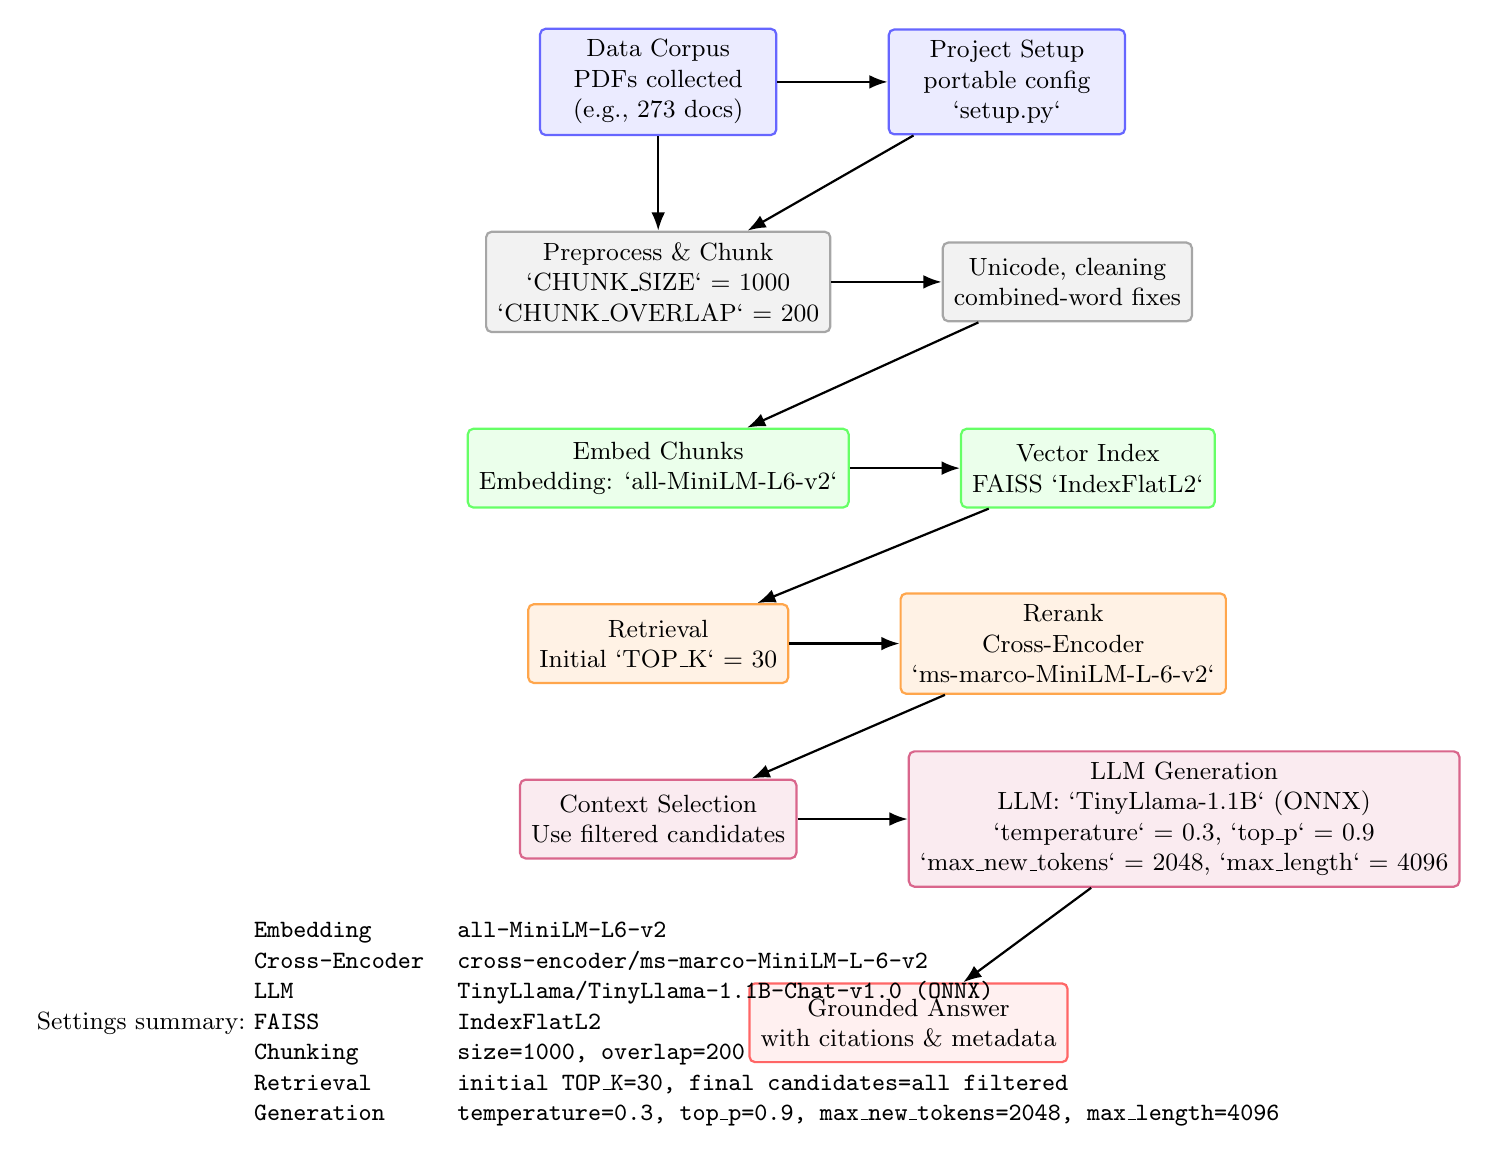
\begin{tikzpicture}[
  font=\small,
  block/.style={draw, rounded corners=2pt, thick, align=center, inner sep=4pt, minimum width=30mm, minimum height=10mm},
  stageA/.style={block, fill=blue!8, draw=blue!60},
  stageB/.style={block, fill=gray!10, draw=gray!70},
  stageC/.style={block, fill=green!8, draw=green!60},
  stageD/.style={block, fill=orange!10, draw=orange!70},
  stageE/.style={block, fill=purple!8, draw=purple!60},
  stageF/.style={block, fill=red!6, draw=red!60},
  line/.style={-Latex, thick}
]

% Row 1: Inputs and Setup
\node[stageA] (pdfs) {Data Corpus\\PDFs collected\\(e.g., 273 docs)};
\node[stageA, right=14mm of pdfs] (setup) {Project Setup\\portable config\\`setup.py`};

% Row 2: Preprocess
\node[stageB, below=12mm of pdfs, xshift=0mm] (chunk) {Preprocess \& Chunk\\`CHUNK\_SIZE` = 1000\\`CHUNK\_OVERLAP` = 200};
\node[stageB, right=14mm of chunk] (clean) {Unicode, cleaning\\combined-word fixes};

% Row 3: Embeddings + Index
\node[stageC, below=12mm of chunk] (embed) {Embed Chunks\\Embedding: `all-MiniLM-L6-v2`};
\node[stageC, right=14mm of embed] (faiss) {Vector Index\\FAISS `IndexFlatL2`};

% Row 4: Retrieval + Rerank
\node[stageD, below=12mm of embed] (retr) {Retrieval\\Initial `TOP\_K` = 30};
\node[stageD, right=14mm of retr] (rerank) {Rerank\\Cross-Encoder\\`ms-marco-MiniLM-L-6-v2`};

% Row 5: Context + Generation
\node[stageE, below=12mm of retr] (context) {Context Selection\\Use filtered candidates};
\node[stageE, right=14mm of context] (llm) {LLM Generation\\LLM: `TinyLlama-1.1B` (ONNX)\\`temperature` = 0.3, `top\_p` = 0.9\\`max\_new\_tokens` = 2048, `max\_length` = 4096};

% Row 6: Output
\node[stageF, below=12mm of llm, xshift=-35mm] (answer) {Grounded Answer\\with citations \& metadata};

% Connections
\draw[line] (pdfs) -- (setup);
\draw[line] (pdfs) -- (chunk);
\draw[line] (setup) -- (chunk);
\draw[line] (chunk) -- (clean);
\draw[line] (clean) -- (embed);
\draw[line] (embed) -- (faiss);
\draw[line] (faiss) -- (retr);
\draw[line] (retr) -- (rerank);
\draw[line] (rerank) -- (context);
\draw[line] (context) -- (llm);
\draw[line] (llm) -- (answer);

% Annotations (bottom legend)
\node[below=6mm of context, align=left] (legend) {Settings summary:~\ttfamily
\begin{tabular}{@{}ll@{}}
Embedding & all-MiniLM-L6-v2 \\
Cross-Encoder & cross-encoder/ms-marco-MiniLM-L-6-v2 \\
LLM & TinyLlama/TinyLlama-1.1B-Chat-v1.0 (ONNX) \\
FAISS & IndexFlatL2 \\
Chunking & size=1000, overlap=200 \\
Retrieval & initial TOP\_K=30, final candidates=all filtered \\
Generation & temperature=0.3, top\_p=0.9, max\_new\_tokens=2048, max\_length=4096 \\
\end{tabular}};

\end{tikzpicture}



% It defines a single tikzpicture environment that draws the complete pipeline.

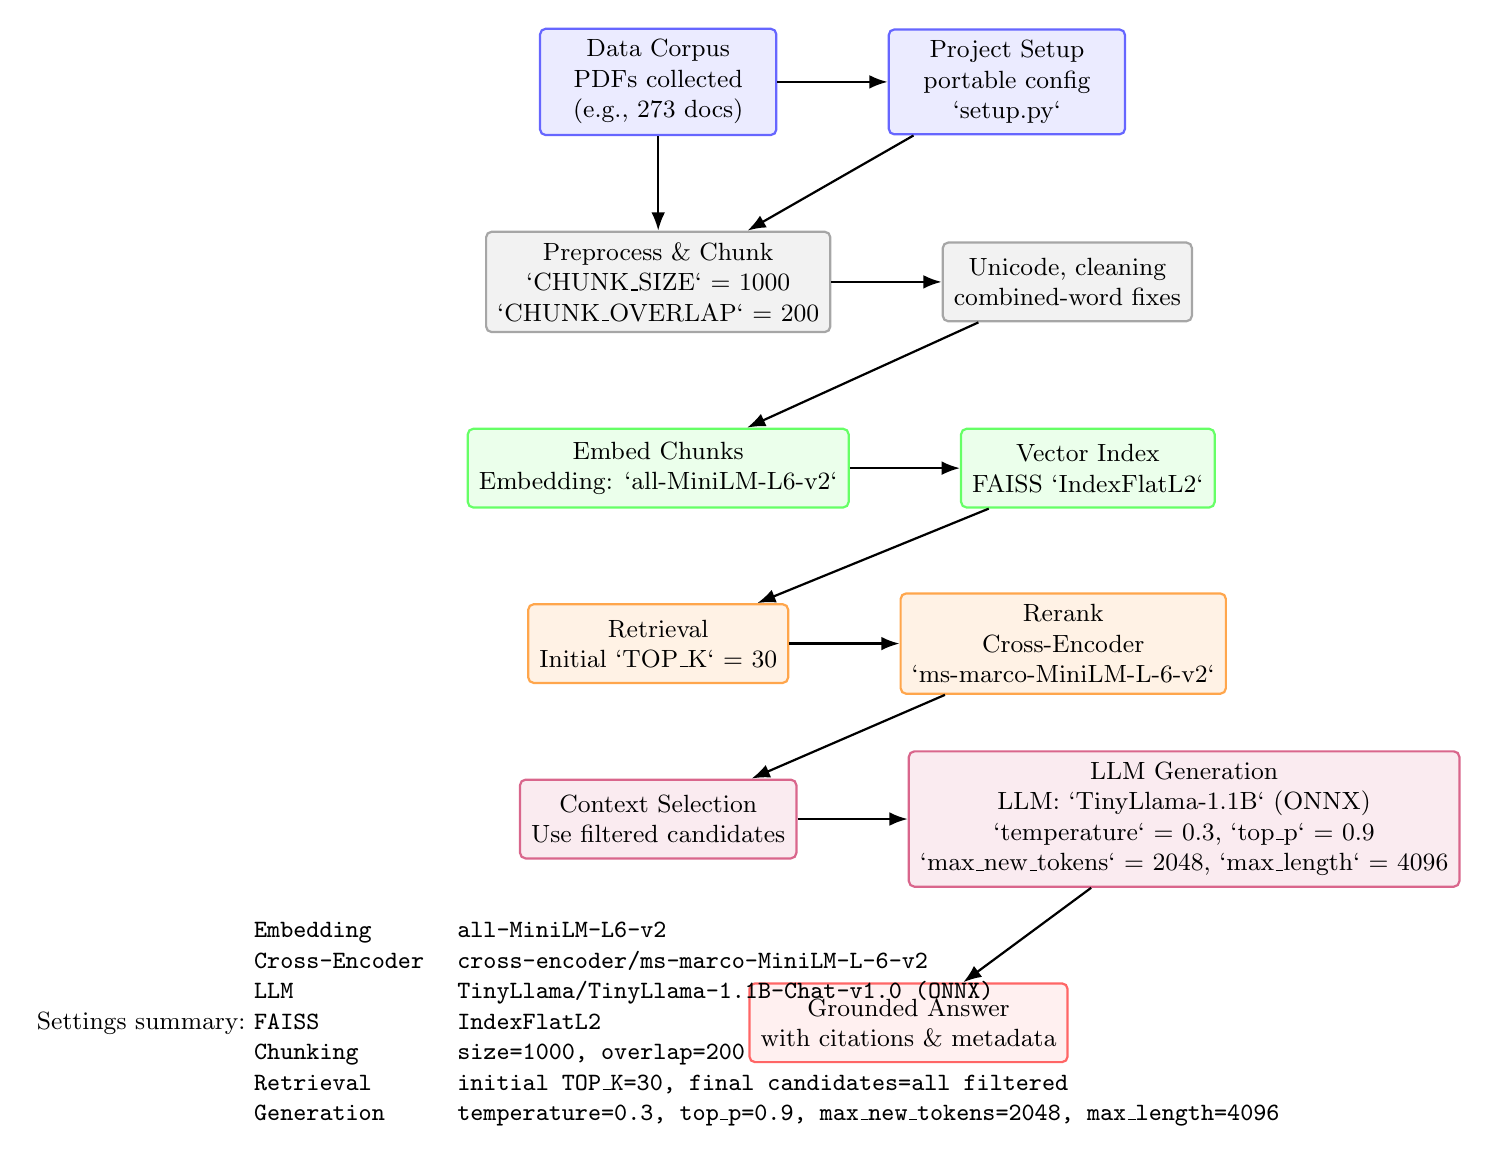
\begin{tikzpicture}[
  font=\small,
  block/.style={draw, rounded corners=2pt, thick, align=center, inner sep=4pt, minimum width=30mm, minimum height=10mm},
  stageA/.style={block, fill=blue!8, draw=blue!60},
  stageB/.style={block, fill=gray!10, draw=gray!70},
  stageC/.style={block, fill=green!8, draw=green!60},
  stageD/.style={block, fill=orange!10, draw=orange!70},
  stageE/.style={block, fill=purple!8, draw=purple!60},
  stageF/.style={block, fill=red!6, draw=red!60},
  line/.style={-Latex, thick}
]

% Row 1: Inputs and Setup
\node[stageA] (pdfs) {Data Corpus\\PDFs collected\\(e.g., 273 docs)};
\node[stageA, right=14mm of pdfs] (setup) {Project Setup\\portable config\\`setup.py`};

% Row 2: Preprocess
\node[stageB, below=12mm of pdfs, xshift=0mm] (chunk) {Preprocess \& Chunk\\`CHUNK\_SIZE` = 1000\\`CHUNK\_OVERLAP` = 200};
\node[stageB, right=14mm of chunk] (clean) {Unicode, cleaning\\combined-word fixes};

% Row 3: Embeddings + Index
\node[stageC, below=12mm of chunk] (embed) {Embed Chunks\\Embedding: `all-MiniLM-L6-v2`};
\node[stageC, right=14mm of embed] (faiss) {Vector Index\\FAISS `IndexFlatL2`};

% Row 4: Retrieval + Rerank
\node[stageD, below=12mm of embed] (retr) {Retrieval\\Initial `TOP\_K` = 30};
\node[stageD, right=14mm of retr] (rerank) {Rerank\\Cross-Encoder\\`ms-marco-MiniLM-L-6-v2`};

% Row 5: Context + Generation
\node[stageE, below=12mm of retr] (context) {Context Selection\\Use filtered candidates};
\node[stageE, right=14mm of context] (llm) {LLM Generation\\LLM: `TinyLlama-1.1B` (ONNX)\\`temperature` = 0.3, `top\_p` = 0.9\\`max\_new\_tokens` = 2048, `max\_length` = 4096};

% Row 6: Output
\node[stageF, below=12mm of llm, xshift=-35mm] (answer) {Grounded Answer\\with citations \& metadata};

% Connections
\draw[line] (pdfs) -- (setup);
\draw[line] (pdfs) -- (chunk);
\draw[line] (setup) -- (chunk);
\draw[line] (chunk) -- (clean);
\draw[line] (clean) -- (embed);
\draw[line] (embed) -- (faiss);
\draw[line] (faiss) -- (retr);
\draw[line] (retr) -- (rerank);
\draw[line] (rerank) -- (context);
\draw[line] (context) -- (llm);
\draw[line] (llm) -- (answer);

% Annotations (bottom legend)
\node[below=6mm of context, align=left] (legend) {Settings summary:~\ttfamily
\begin{tabular}{@{}ll@{}}
Embedding & all-MiniLM-L6-v2 \\
Cross-Encoder & cross-encoder/ms-marco-MiniLM-L-6-v2 \\
LLM & TinyLlama/TinyLlama-1.1B-Chat-v1.0 (ONNX) \\
FAISS & IndexFlatL2 \\
Chunking & size=1000, overlap=200 \\
Retrieval & initial TOP\_K=30, final candidates=all filtered \\
Generation & temperature=0.3, top\_p=0.9, max\_new\_tokens=2048, max\_length=4096 \\
\end{tabular}};

\end{tikzpicture}



% It defines a single tikzpicture environment that draws the complete pipeline.

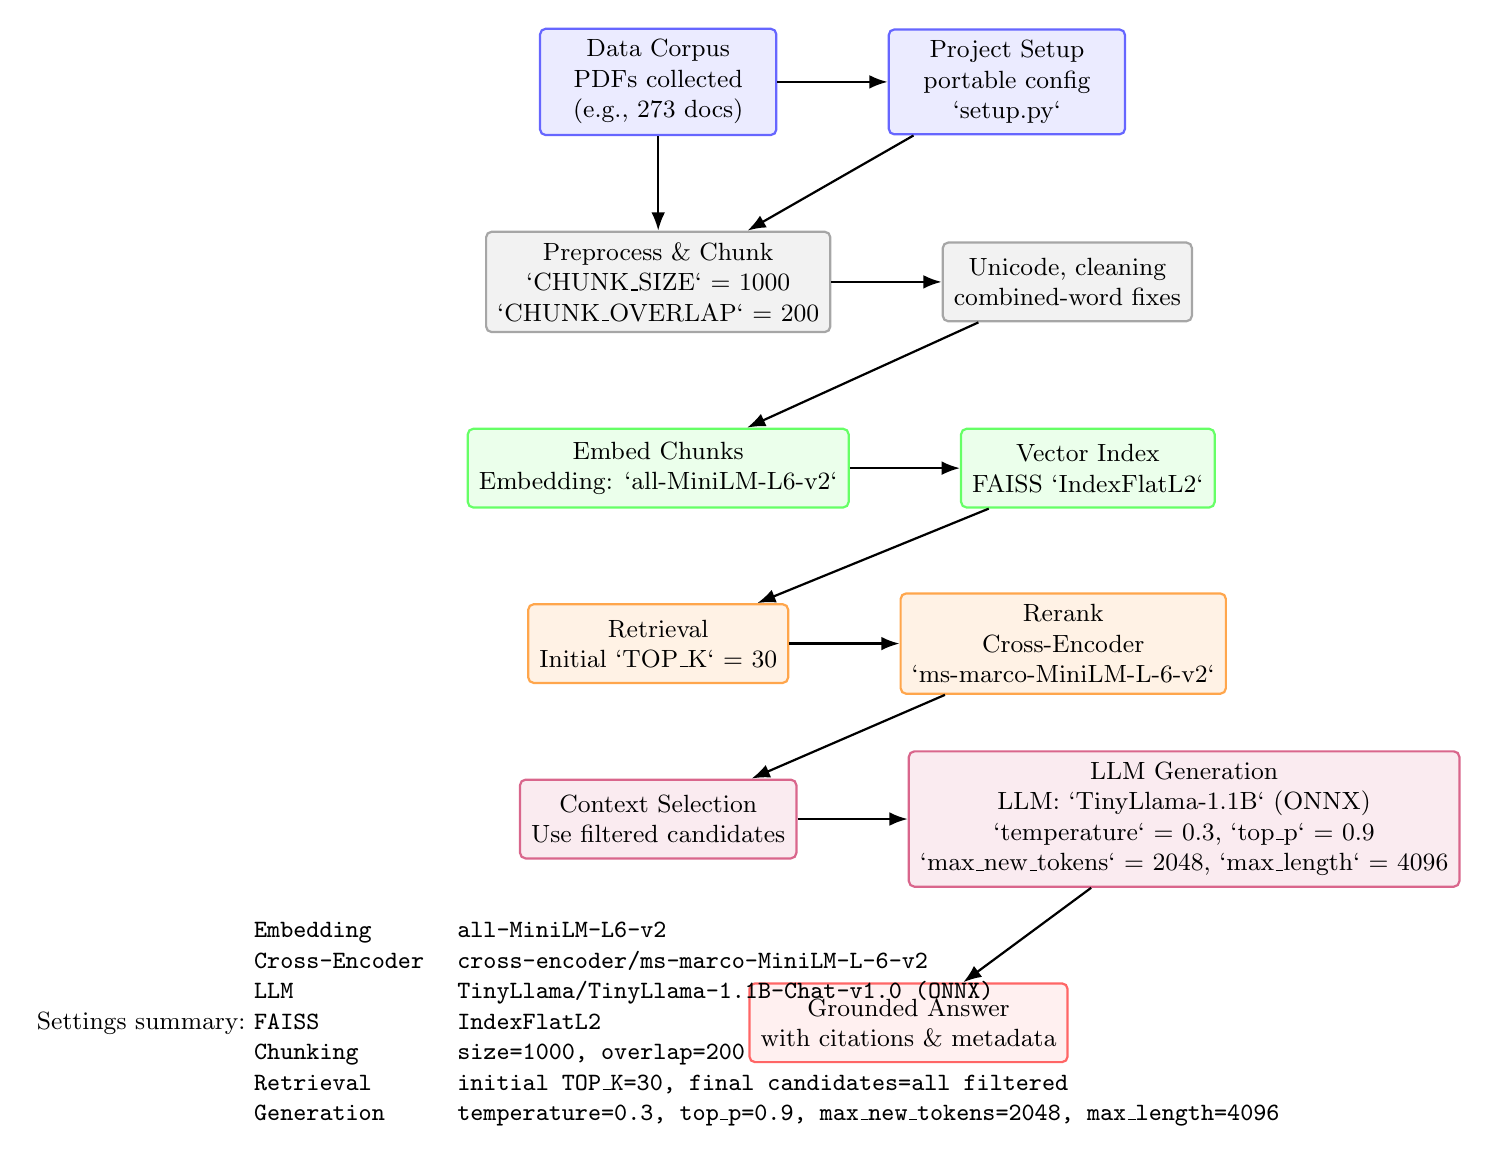
\begin{tikzpicture}[
  font=\small,
  block/.style={draw, rounded corners=2pt, thick, align=center, inner sep=4pt, minimum width=30mm, minimum height=10mm},
  stageA/.style={block, fill=blue!8, draw=blue!60},
  stageB/.style={block, fill=gray!10, draw=gray!70},
  stageC/.style={block, fill=green!8, draw=green!60},
  stageD/.style={block, fill=orange!10, draw=orange!70},
  stageE/.style={block, fill=purple!8, draw=purple!60},
  stageF/.style={block, fill=red!6, draw=red!60},
  line/.style={-Latex, thick}
]

% Row 1: Inputs and Setup
\node[stageA] (pdfs) {Data Corpus\\PDFs collected\\(e.g., 273 docs)};
\node[stageA, right=14mm of pdfs] (setup) {Project Setup\\portable config\\`setup.py`};

% Row 2: Preprocess
\node[stageB, below=12mm of pdfs, xshift=0mm] (chunk) {Preprocess \& Chunk\\`CHUNK\_SIZE` = 1000\\`CHUNK\_OVERLAP` = 200};
\node[stageB, right=14mm of chunk] (clean) {Unicode, cleaning\\combined-word fixes};

% Row 3: Embeddings + Index
\node[stageC, below=12mm of chunk] (embed) {Embed Chunks\\Embedding: `all-MiniLM-L6-v2`};
\node[stageC, right=14mm of embed] (faiss) {Vector Index\\FAISS `IndexFlatL2`};

% Row 4: Retrieval + Rerank
\node[stageD, below=12mm of embed] (retr) {Retrieval\\Initial `TOP\_K` = 30};
\node[stageD, right=14mm of retr] (rerank) {Rerank\\Cross-Encoder\\`ms-marco-MiniLM-L-6-v2`};

% Row 5: Context + Generation
\node[stageE, below=12mm of retr] (context) {Context Selection\\Use filtered candidates};
\node[stageE, right=14mm of context] (llm) {LLM Generation\\LLM: `TinyLlama-1.1B` (ONNX)\\`temperature` = 0.3, `top\_p` = 0.9\\`max\_new\_tokens` = 2048, `max\_length` = 4096};

% Row 6: Output
\node[stageF, below=12mm of llm, xshift=-35mm] (answer) {Grounded Answer\\with citations \& metadata};

% Connections
\draw[line] (pdfs) -- (setup);
\draw[line] (pdfs) -- (chunk);
\draw[line] (setup) -- (chunk);
\draw[line] (chunk) -- (clean);
\draw[line] (clean) -- (embed);
\draw[line] (embed) -- (faiss);
\draw[line] (faiss) -- (retr);
\draw[line] (retr) -- (rerank);
\draw[line] (rerank) -- (context);
\draw[line] (context) -- (llm);
\draw[line] (llm) -- (answer);

% Annotations (bottom legend)
\node[below=6mm of context, align=left] (legend) {Settings summary:~\ttfamily
\begin{tabular}{@{}ll@{}}
Embedding & all-MiniLM-L6-v2 \\
Cross-Encoder & cross-encoder/ms-marco-MiniLM-L-6-v2 \\
LLM & TinyLlama/TinyLlama-1.1B-Chat-v1.0 (ONNX) \\
FAISS & IndexFlatL2 \\
Chunking & size=1000, overlap=200 \\
Retrieval & initial TOP\_K=30, final candidates=all filtered \\
Generation & temperature=0.3, top\_p=0.9, max\_new\_tokens=2048, max\_length=4096 \\
\end{tabular}};

\end{tikzpicture}



\end{center}

\section{Methods}
\subsection{Document Processing}
Corpus PDFs are normalized and chunked with page-aware boundaries. Unicode analysis and combined-word postprocessing improve downstream embedding quality. Parameters: `CHUNK\_SIZE=1000`, `CHUNK\_OVERLAP=200`.

\subsection{Embedding and Indexing}
Text chunks are encoded with `all-MiniLM-L6-v2` (384-dim) and stored in a FAISS `IndexFlatL2` structure. Metadata is preserved for citation.

\subsection{Retrieval and Re-ranking}
Initial retrieval returns up to `TOP\_K=30` candidates via FAISS. Cross-encoder `ms-marco-MiniLM-L-6-v2` re-ranks candidates; contextual keyword filtering removes low-signal chunks. All remaining filtered candidates are passed to the generator to avoid arbitrary truncation.

\subsection{Controlled Generation}
The generator defaults to TinyLlama 1.1B (ONNX-optimized when available) with temperature `0.3`, top-p `0.9`, and token limits `max\_length=4096`, `max\_new\_tokens=2048`. A conservative prompt template encourages concise, practical responses with minimal citations and explicit acknowledgement of uncertainty when sources are insufficient.

\section{Implementation Details}
Core modules include `scaffold\_core/vector/enhanced\_query\_improved.py` (hybrid retrieval and prompt construction), `scaffold\_core/llm.py` (LLM manager with continuation support), and `scaffold\_core/config.py` (central configuration, model registries, environment keys). The UI layer provides model selection and parameter controls; however, this report focuses on the headless RAG core.

\section{Evaluation Summary}
Internal tests indicate: (i) stable citation rendering with preserved metadata, (ii) reduced repetition relative to earlier prompts, and (iii) robust behavior under variable query difficulty. Performance is CPU-feasible due to compact models; GPU acceleration is optional. Detailed quantitative benchmarks (latency, memory) are tracked separately in repository logs.

\section{Limitations}
The compact LLM constrains depth of synthesis on complex queries. Citation granularity (e.g., page spans) is limited by source metadata. Some domain-specific terminology may require larger context windows or specialized models.

\section{Reproducibility Settings}
\begin{longtable}{@{}ll@{}}
\toprule
Component & Setting \\
\midrule
Embedding model & \texttt{all-MiniLM-L6-v2} \\
Cross-encoder & \texttt{cross-encoder/ms-marco-MiniLM-L-6-v2} \\
LLM & \texttt{TinyLlama/TinyLlama-1.1B-Chat-v1.0} (ONNX when available) \\
Chunk size / overlap & 1000 / 200 \\
FAISS index & \texttt{IndexFlatL2} \\
Initial retrieval & \texttt{TOP\_K=30} \\
Final candidates & All filtered (no fixed cut) \\
Temperature / top-p & 0.3 / 0.9 \\
Max length / new tokens & 4096 / 2048 \\
\bottomrule
\end{longtable}

\section{Conclusion}
Scaffold AI demonstrates that a carefully engineered compact RAG stack can provide literature-grounded curriculum recommendations suitable for early-stage adoption in engineering courses. The present configuration prioritizes transparency, determinism, and operational feasibility, while leaving room for future upgrades to larger models and richer citation features.

\section*{Availability}
Source code, configuration, and evaluation artifacts are available within the repository. Execution requires Python 3.11+ and the dependencies listed in \texttt{requirements.txt}. Optional hardware acceleration is automatically detected.

\end{document}


